\documentclass[11pt,letterpaper]{article}
\usepackage[top=0.85in,bottom=0.85in,left=1in,right=1in]{geometry}
\usepackage{amsmath,amssymb}
\usepackage{xcolor}
\usepackage{mdframed}
\usepackage{booktabs}
\usepackage{fancyhdr}
\usepackage{cancel}
\usepackage{array}
\usepackage{tikz}

% ── Colors ──
\definecolor{purple}{HTML}{534AB7}\definecolor{purplebg}{HTML}{EEEDFE}
\definecolor{teal}{HTML}{0F6E56}\definecolor{tealbg}{HTML}{E1F5EE}
\definecolor{coral}{HTML}{993C1D}\definecolor{coralbg}{HTML}{FAECE7}

% Cheat-sheet reference tag
\newcommand{\cs}[1]{\textcolor{teal}{\footnotesize[CS\,#1]}}

% Question text box (gray)
\newmdenv[linewidth=0.6pt,linecolor=black!35,backgroundcolor=black!4,
  innerleftmargin=8pt,innerrightmargin=8pt,
  innertopmargin=6pt,innerbottommargin=6pt,
  skipabove=5pt,skipbelow=5pt]{qbox}

% Cheat-sheet snippet box (teal)
\newmdenv[linewidth=1pt,linecolor=teal,backgroundcolor=tealbg!30,
  innerleftmargin=6pt,innerrightmargin=6pt,
  innertopmargin=5pt,innerbottommargin=5pt,
  skipabove=5pt,skipbelow=5pt]{cssnip}

% Warning box (coral)
\newmdenv[linewidth=1pt,linecolor=coral,backgroundcolor=coralbg!40,
  innerleftmargin=6pt,innerrightmargin=6pt,
  innertopmargin=4pt,innerbottommargin=4pt,
  skipabove=4pt,skipbelow=4pt]{notebox}

\pagestyle{fancy}\fancyhf{}
\renewcommand{\headrulewidth}{0.4pt}
\fancyhead[L]{\textbf{ECE332 Fall 2025 --- Exam 1 Answer Key (Alternative --- Flux Linkage Q1a)}}
\fancyhead[R]{Bao Nguyen}
\fancyfoot[C]{\thepage}

\setlength{\parindent}{0pt}
\setlength{\parskip}{4pt}

\begin{document}

%══════════════════════════════════════════════════════════════════════
% COVER
%══════════════════════════════════════════════════════════════════════
\begin{center}
{\Large\textbf{ECE 332 Fall 2025 --- Exam 1 Answer Key (Alternative)}}\\[4pt]
{\normalsize\textit{Variant: Q1(a) asks for total flux linkage $\Lambda=N\Phi$ instead of single-turn flux}}\\[6pt]
{\small\textcolor{teal}{[CS\,p.1]} = page 1 of cheat sheet \quad
       \textcolor{teal}{[CS\,p.2]} = page 2}
\end{center}

\vspace{4pt}
\begin{notebox}
\textbf{\textcolor{coral}{Two corrected errors from prior keys:}}\\[2pt]
\textbf{(1) Q1(c):} Exam writes ``$\omega=2\,\text{MHz}$'' but MHz is a frequency unit.
Must convert: $\omega=2\pi f=2\pi\times2\times10^6=4\pi\times10^6\,\text{rad/s}$.\\[2pt]
\textbf{(2) Q6:} Exam gives $f=\tfrac{2}{\pi}\,\text{GHz}$ (not $\tfrac{2}{5}$\,GHz).
$\omega=2\pi f=2\pi\cdot\tfrac{2}{\pi}\times10^9=4\times10^9\,\text{rad/s}$.
\end{notebox}

\vspace{6pt}
\begin{center}
\renewcommand{\arraystretch}{1.3}
\begin{tabular}{@{}lccc@{}}
\toprule
Question & Topic & Points & Page\\
\midrule
Q1 & Triangular loop EMF (flux linkage variant) & 20 & 2\\
Q2 & Moving wire (motional EMF) & 12 & 3\\
Q3 & Conduction \& displacement current & 12 & 4\\
Q4 & Charge relaxation & 10 & 5\\
Q5 & Lossless plane wave & 30 & 6\\
Q6 & Lossy wave in distilled water & 16 & 8\\
\midrule
 & \textbf{Total} & \textbf{100} &\\
\bottomrule
\end{tabular}
\end{center}

\newpage
%══════════════════════════════════════════════════════════════════════
% QUESTION 1
%══════════════════════════════════════════════════════════════════════
\colorbox{purplebg}{\parbox{\dimexpr\linewidth-2\fboxsep}{\color{purple}\large\textbf{Question 1 --- Triangular Loop \hfill 20 pts}}}

\begin{qbox}
Suppose an equilateral triangular conducting loop of $N$ turns with sides of length $a$ is located in the $y$-$z$ plane with normal $d\mathbf{s}=\hat{x}\,ds$, as shown below, in a magnetic field
\[
\mathbf{B}(t)=B_0(-2\hat{x}+3\hat{y})\sin(\omega t).
\]
\begin{center}
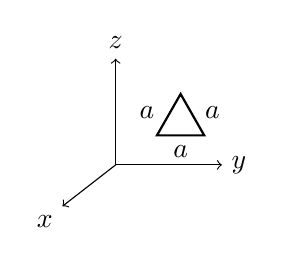
\begin{tikzpicture}[scale=0.75]
\draw[->] (0,0,0) -- (1.8,0,0) node[right]{$y$};
\draw[->] (0,0,0) -- (0,1.8,0) node[above]{$z$};
\draw[->] (0,0,0) -- (-0.9,-0.7,0) node[below left]{$x$};
\draw[thick] (0.7,0.5) -- (1.5,0.5) -- (1.1,1.2) -- cycle;
\node[below] at (1.1,0.5) {$a$};
\node[left]  at (0.82,0.88) {$a$};
\node[right] at (1.35,0.88) {$a$};
\end{tikzpicture}
\end{center}
\textbf{(a)} Find a formula for the total magnetic flux linkage $\Lambda$ through $N$ turns of the loop.\hfill\textit{(6 pts)}\\[3pt]
\textbf{(b)} Find a formula for the emf induced in the loop at time $t$.\hfill\textit{(6 pts)}\\[3pt]
\textbf{(c)} Determine the current flowing through a $1\,\text{k}\Omega$ resistor incorporated in the loop when $N=10$, $a=8\,\text{cm}$, $B_0=0.02\,\text{T}$, $\omega=2\,\text{MHz}$, and $\omega t=\pi/4$, assuming that the resistance of the loop material is negligible.\hfill\textit{(8 pts)}
\end{qbox}

\begin{cssnip}
\textbf{\small\textcolor{teal}{Cheat Sheet Snippets (p.1)}}\\[3pt]
\begin{tabular}{@{}p{0.47\linewidth}p{0.47\linewidth}@{}}
\textbf{EMF \& FARADAY'S LAW} & \textbf{SURFACE ELEMENT}\\
$V_\text{emf}=-\dfrac{d\Lambda}{dt}$,\; $\Lambda=N\Phi$,\; $\Phi=\displaystyle\int_S\mathbf{B}\cdot d\mathbf{s}$ &
$y$-$z$ plane $\Rightarrow d\mathbf{s}=\hat{x}\,da$\\[5pt]
\textbf{DOT PRODUCTS} & \textbf{EQUILATERAL TRIANGLE}\\
$\hat{x}\cdot\hat{x}=1$,\quad $\hat{y}\cdot\hat{x}=0$ & Area (side $a$): $A=\dfrac{\sqrt{3}}{4}a^2$\\[5pt]
\textbf{$\partial B/\partial t$ TABLE} & \textbf{CIRCUIT \& WAVE + UNIT CIRCLE}\\
$\dfrac{d}{dt}\sin(\omega t)=\omega\cos(\omega t)$ & $\omega=2\pi f$;\quad $\cos(\pi/4)=\dfrac{\sqrt{2}}{2}$\\
\end{tabular}
\end{cssnip}

\textbf{(a)} First find the single-turn flux:
\[
\Phi=\int_S B_0(-2\hat{x}+3\hat{y})\sin(\omega t)\cdot\hat{x}\,da
=A\!\left(-2(\hat{x}\cdot\hat{x})+3(\hat{y}\cdot\hat{x})\right)B_0\sin(\omega t)
=-2\cdot\tfrac{\sqrt{3}}{4}a^2 B_0\sin(\omega t)
=-\tfrac{\sqrt{3}}{2}B_0 a^2\sin(\omega t)
\]
The total flux linkage through $N$ turns is $\Lambda=N\Phi$:
\[\boxed{\Lambda=N\Phi=-\tfrac{\sqrt{3}}{2}N B_0 a^2\sin(\omega t)\;\text{V$\cdot$s}}\]

\textbf{(b)} Since $\Lambda$ already contains $N$, differentiate directly --- no extra $N$ factor:
\[V_\text{emf}=-\frac{d\Lambda}{dt}=-\frac{d}{dt}\!\left(-\tfrac{\sqrt{3}}{2}N B_0 a^2\sin(\omega t)\right)
\qquad\boxed{V_\text{emf}(t)=\tfrac{\sqrt{3}}{2}N B_0 a^2\omega\cos(\omega t)\;\text{V}}\]

\textbf{(c)}
\begin{notebox}
Exam says ``$\omega=2\,\text{MHz}$'' $\Rightarrow$ convert: $\omega=2\pi f=2\pi(2\times10^6)=4\pi\times10^6\,\text{rad/s}$
\end{notebox}
\[|V_\text{emf}|=\tfrac{\sqrt{3}}{2}(10)(0.02)(0.08)^2(4\pi\times10^6)\underbrace{\cos(\pi/4)}_{\sqrt{2}/2}=9.85\times10^3\;\text{V}\]
\[I=\frac{V_\text{emf}}{R}=\frac{9.85\;\text{kV}}{1000\;\Omega}\qquad\boxed{I\approx9.85\;\text{A}}\]

\newpage
%══════════════════════════════════════════════════════════════════════
% QUESTION 2
%══════════════════════════════════════════════════════════════════════
\colorbox{purplebg}{\parbox{\dimexpr\linewidth-2\fboxsep}{\color{purple}\large\textbf{Question 2 --- Moving Wire \hfill 12 pts}}}

\begin{qbox}
A straight conducting wire of length $a=15\,\text{cm}$ lying along the $\hat{y}$ direction moves with velocity $\mathbf{u}=12\hat{x}\,\text{cm/s}$ in a magnetic field
\[\mathbf{B}=(0.1\hat{x}-0.05\hat{z})\;\text{T}.\]
Find the emf between the two ends of the wire.\hfill\textit{(12 pts)}
\end{qbox}

\begin{cssnip}
\textbf{\small\textcolor{teal}{Cheat Sheet Snippets (p.1)}}\\[3pt]
\begin{tabular}{@{}p{0.47\linewidth}p{0.47\linewidth}@{}}
\textbf{EMF \& FARADAY'S LAW (Motional)} & \textbf{CROSS PRODUCT cycle}\\
$V_\text{emf}=\displaystyle\oint(\mathbf{u}\times\mathbf{B})\cdot d\mathbf{l}$ &
$\hat{x}\times\hat{z}=-\hat{y}$ (reversed cycle)\\
$d\mathbf{l}=\hat{y}\,dy$ along $\hat{y}$-wire & $\hat{x}\times\hat{x}=0$
\end{tabular}
\end{cssnip}

$a=0.15\,\text{m}$,\quad $\mathbf{u}=0.12\hat{x}\,\text{m/s}$.

\[\mathbf{u}\times\mathbf{B}=0.12\hat{x}\times(0.1\hat{x}-0.05\hat{z})
=0.012\underbrace{(\hat{x}\times\hat{x})}_{0}+(-0.006)\underbrace{(\hat{x}\times\hat{z})}_{-\hat{y}}
=6\times10^{-3}\hat{y}\;\text{V/m}\]
\[V_\text{emf}=\int_0^{0.15}6\times10^{-3}\,dy=6\times10^{-3}(0.15)
\qquad\boxed{V_\text{emf}=900\;\mu\text{V}=0.9\;\text{mV}}\]

\newpage
%══════════════════════════════════════════════════════════════════════
% QUESTION 3
%══════════════════════════════════════════════════════════════════════
\colorbox{coralbg}{\parbox{\dimexpr\linewidth-2\fboxsep}{\color{coral}\large\textbf{Question 3 --- Conduction \& Displacement Current \hfill 12 pts}}}

\begin{qbox}
Suppose a total conduction current $I_c=2\sin(\omega t)\,\mu\text{A}$ flows through a column of distilled water with cross-sectional area $A$ in a glass tube. Distilled water has conductivity $\sigma\approx10^{-4}\,\text{S/m}$ and relative permittivity $\varepsilon_r\approx26\pi$, and the current flowing through the glass is negligible.\\[4pt]
\textbf{(a)} Use the relationship between the conduction current, the current density, the cross-sectional area, and Ohm's law to determine the electric field intensity $E$ at a cross-section of the water.\hfill\textit{(6 pts)}\\[3pt]
\textbf{(b)} Determine the displacement current $I_d$ through the cross-section when the angular frequency of $I_c$ is $\omega=10^9\,\text{rad\,s}^{-1}$ and $\omega t=\pi/3$.\hfill\textit{(6 pts)}
\end{qbox}

\begin{cssnip}
\textbf{\small\textcolor{teal}{Cheat Sheet Snippets (p.1)}}\\[3pt]
\begin{tabular}{@{}p{0.60\linewidth}p{0.35\linewidth}@{}}
\textbf{DISPLACEMENT \& CONDUCTION CURRENT} & \textbf{UNIT CIRCLE}\\
$E=V(t)/d$\quad $I_c=\dfrac{\sigma A}{d}V(t)$\quad $J_c=\sigma E$ & $\cos(\pi/3)=\dfrac{1}{2}$\\[4pt]
$I_d=C\dfrac{dV}{dt}$\quad $C=\dfrac{\varepsilon_r\varepsilon_0 A}{d}$\quad $J_d=\varepsilon\dfrac{\partial E}{\partial t}$ &
\end{tabular}
\end{cssnip}

\textbf{(a)}
\[E=\frac{V(t)}{d},\qquad I_c=\frac{\sigma A}{d}V(t)\;\Rightarrow\;V(t)=\frac{I_c\,d}{\sigma A}
\qquad E=\frac{I_c}{\sigma A}=\frac{2\times10^{-6}\sin(\omega t)}{10^{-4}A}
\qquad\boxed{E=\frac{0.02}{A}\sin(\omega t)\;\text{V/m}}\]

\textbf{(b)} From (a): $V(t)=E\cdot d=\dfrac{d\cdot0.02}{A}\sin(\omega t)$.
\[I_d=\frac{\varepsilon_r\varepsilon_0 A}{d}\cdot\frac{dV}{dt}
=\frac{\varepsilon_r\varepsilon_0\cancel{A}}{\cancel{d}}\cdot\frac{\cancel{d}\cdot0.02}{\cancel{A}}\cdot\omega\cos(\omega t)
=\varepsilon_r\varepsilon_0\cdot0.02\cdot\omega\cos(\omega t)\]
At $\omega t=\pi/3$, $\cos(\pi/3)=\tfrac{1}{2}$:
\[I_d=(26\pi)(8.85\times10^{-12})(0.02)(10^9)\!\left(\tfrac{1}{2}\right)
\qquad\boxed{I_d\approx7.23\;\text{mA}}\]

\newpage
%══════════════════════════════════════════════════════════════════════
% QUESTION 4
%══════════════════════════════════════════════════════════════════════
\colorbox{coralbg}{\parbox{\dimexpr\linewidth-2\fboxsep}{\color{coral}\large\textbf{Question 4 --- Charge Relaxation \hfill 10 pts}}}

\begin{qbox}
Distilled water has a conductivity $\sigma\approx10^{-4}\,\text{S/m}$ and $\varepsilon_r\approx26\pi$.\\[4pt]
\textbf{(a)} Find the relaxation time constant for distilled water.\hfill\textit{(5 pts)}\\[3pt]
\textbf{(b)} How long does it take for an excess charge density in distilled water to decay to $e^{-3}$ times its initial value?\hfill\textit{(5 pts)}
\end{qbox}

\begin{cssnip}
\textbf{\small\textcolor{teal}{Cheat Sheet Snippet (p.1 --- CHARGE RELAXATION)}}
\[\tau_r=\frac{\varepsilon_r\varepsilon_0}{\sigma}\qquad\qquad\rho_v(t)=\rho_{v0}\,e^{-t/\tau_r}\]
\end{cssnip}

\textbf{(a)}
\[\tau_r=\frac{\varepsilon_r\varepsilon_0}{\sigma}=\frac{(26\pi)(8.85\times10^{-12})}{10^{-4}}
\qquad\boxed{\tau_r\approx7.23\;\mu\text{s}}\]

\textbf{(b)} Set $\rho_{v0}\,e^{-3}=\rho_{v0}\,e^{-t/\tau_r}$ and take $\ln$:
\[\ln e^{-3}=\frac{-t}{\tau_r}\;\Rightarrow\;t=-\tau_r\ln(e^{-3})=3\tau_r
\qquad\boxed{t=3\times7.23\;\mu\text{s}\approx21.69\;\mu\text{s}}\]

\newpage
%══════════════════════════════════════════════════════════════════════
% QUESTION 5
%══════════════════════════════════════════════════════════════════════
\colorbox{purplebg}{\parbox{\dimexpr\linewidth-2\fboxsep}{\color{purple}\large\textbf{Question 5 --- Lossless Plane Wave \hfill 30 pts}}}

\begin{qbox}
Suppose the electric field intensity of an EM wave in a nonconducting, source-free medium with $\varepsilon_r=6$ and $\mu_r=1$ is
\[\mathbf{E}(z,t)=4\cos\!\left((6\pi\times10^8\,\text{rad/s})\,t-kz-\frac{\pi}{6}\right)\hat{y}\;\text{V/m}.\]
\textbf{(a)} Determine $\omega$, $k$, $\lambda$, and $\eta$.\hfill\textit{(10 pts)}\\[2pt]
\textbf{(b)} Find $\tilde{\mathbf{E}}(z)$.\hfill\textit{(5 pts)}\\[2pt]
\textbf{(c)} Find $\tilde{\mathbf{H}}(z)$.\hfill\textit{(5 pts)}\\[2pt]
\textbf{(d)} Determine the magnetic field intensity $\mathbf{H}(z,t)$.\hfill\textit{(5 pts)}\\[2pt]
\textbf{(e)} Determine the average power density that the EM wave carries.\hfill\textit{(5 pts)}
\end{qbox}

\begin{cssnip}
\textbf{\small\textcolor{teal}{Cheat Sheet Snippets}}\\[3pt]
\begin{tabular}{@{}p{0.47\linewidth}p{0.47\linewidth}@{}}
\textbf{WAVE PARAMS (p.2 strip)} & \textbf{DIRECTION OF PROP.\ (p.2)}\\
$k=\omega\sqrt{\mu_r\mu_0\varepsilon_r\varepsilon_0}$,\; $\lambda=2\pi/k$ &
$-kz$ in arg $\Rightarrow\hat{k}=+\hat{z}$\\[3pt]
$\eta=\eta_0/\sqrt{\varepsilon_r}=377/\sqrt{\varepsilon_r}$ &
\textbf{$\hat{k}\times\hat{E}$ TABLE (p.2):} $+\hat{z}$, $\hat{y}\Rightarrow-\hat{x}$\\[3pt]
\textbf{PHASOR METHOD (p.1)} & \textbf{LOSSLESS E\,\&\,H (p.2)}\\
$\mathbf{E}=\operatorname{Re}\!\{\tilde{\mathbf{E}}\,e^{j\omega t}\}$; strip $e^{j\omega t}$ &
$\tilde{\mathbf{H}}=\tfrac{1}{\eta}(\hat{k}\times\tilde{\mathbf{E}})$\\[3pt]
\textbf{PHASOR $\leftrightarrow$ TIME (p.2)} & \textbf{POYNTING lossless (p.2)}\\
$\operatorname{Re}\!\{Ae^{j(\omega t-\beta z+\phi)}\}=A\cos(\omega t-\beta z+\phi)$ &
$\mathbf{S}_\text{av}=\tfrac{|E_0|^2}{2\eta}\hat{k}$\\
\end{tabular}
\end{cssnip}

\textbf{(a)}
\[\boxed{\omega=6\pi\times10^8\;\text{rad/s}}\qquad
k=(6\pi\times10^8)\sqrt{(4\pi\times10^{-7})(6)(8.85\times10^{-12})}\quad\boxed{k\approx15.40\;\text{rad/m}}\]
\[\lambda=\frac{2\pi}{15.40}\quad\boxed{\lambda\approx0.408\;\text{m}}\qquad\qquad
\eta=\frac{377}{\sqrt{6}}\quad\boxed{\eta\approx153.91\;\Omega}\]

\textbf{(b)} Let $\phi=\pi/6$. Strip $e^{j\omega t}$: $\tilde{\mathbf{E}}=4\,e^{j(-kz-\phi)}\hat{y}$.
\[\boxed{\tilde{\mathbf{E}}(z)=4\,e^{-j(15.40\,z+\pi/6)}\hat{y}\;\text{V/m}}\]

\textbf{(c)} $\hat{k}=+\hat{z}$;\quad $\hat{z}\times\hat{y}=-\hat{x}$:
\[\tilde{\mathbf{H}}=\tfrac{1}{\eta}(\hat{z}\times\tilde{\mathbf{E}})
=-\tfrac{4}{153.91}\,e^{-j(15.40z+\pi/6)}\hat{x}
\qquad\boxed{\tilde{\mathbf{H}}(z)\approx-25.99\times10^{-3}e^{-j(15.40z+\pi/6)}\hat{x}\;\text{A/m}}\]

\newpage

\colorbox{purplebg}{\parbox{\dimexpr\linewidth-2\fboxsep}{\color{purple}\large\textbf{Question 5 (continued)}}}

\vspace{6pt}
\textbf{(d)}
\begin{align*}
\mathbf{H}(z,t)&=\operatorname{Re}\!\left\{-25.99\times10^{-3}e^{-j(15.40z+\pi/6)}\hat{x}\cdot e^{j\omega t}\right\}\\
&=\operatorname{Re}\!\left\{-25.99\times10^{-3}e^{j(\omega t-15.40z-\pi/6)}\hat{x}\right\}
\end{align*}
\[\boxed{\mathbf{H}(z,t)=-25.99\times10^{-3}\cos\!\left(6\pi\times10^8 t-15.40\,z-\tfrac{\pi}{6}\right)\hat{x}\;\text{A/m}}\]

\textbf{(e)} Lossless $\Rightarrow$
\[\mathbf{S}_\text{av}=\frac{|E_0|^2}{2\eta}\hat{z}=\frac{4^2}{2(153.91)}\hat{z}
\qquad\boxed{\mathbf{S}_\text{av}\approx51.98\times10^{-3}\,\hat{z}\;\text{W/m}^2}\]

\newpage
%══════════════════════════════════════════════════════════════════════
% QUESTION 6
%══════════════════════════════════════════════════════════════════════
\colorbox{coralbg}{\parbox{\dimexpr\linewidth-2\fboxsep}{\color{coral}\large\textbf{Question 6 --- EM Wave in Distilled Water \hfill 16 pts}}}

\begin{qbox}
Consider a $\tfrac{2}{\pi}\,\text{GHz}$ EM wave traveling in distilled water, where $\sigma\approx10^{-4}\,\text{S/m}$, $\varepsilon_r\approx26\pi$, and $\mu_r=1$. The wave travels downward into the water, where the $+z$ direction is down and $z=0$ is just below the surface. The amplitude of the electric field at the surface is $4\,\text{V/m}$.\\[4pt]
\textbf{(a)} Find $\varepsilon''/\varepsilon'$.\hfill\textit{(6 pts)}\\[2pt]
\textbf{(b)} What type of medium is distilled water at this frequency? Justify your answer.\hfill\textit{(5 pts)}\\[2pt]
\textbf{(c)} Find the skin depth for distilled water at this frequency.\hfill\textit{(5 pts)}
\end{qbox}

\begin{cssnip}
\textbf{\small\textcolor{teal}{Cheat Sheet Snippets (p.2)}}\\[3pt]
\begin{tabular}{@{}p{0.47\linewidth}p{0.47\linewidth}@{}}
\textbf{WAVE PARAMS strip} & \textbf{LOSSY MEDIA --- CLASSIFICATION}\\
$\omega=2\pi f$\quad $\eta=377/\sqrt{\varepsilon_r}$ &
$\varepsilon''/\varepsilon'=\sigma/(\omega\varepsilon_r\varepsilon_0)$\\[3pt]
\textbf{SKIN DEPTH --- LOW-LOSS MEDIUM} & $<0.01\Rightarrow$ low-loss dielectric\\
$\delta_s=2/(\sigma\eta)$ \textit{(from $\alpha=\sigma\eta/2$)} & \\
\end{tabular}
\end{cssnip}

\begin{notebox}
$\omega=2\pi f=2\pi\cdot\dfrac{2}{\pi}\times10^9=4\times10^9\;\text{rad/s}$
\end{notebox}

\textbf{(a)}
\[\frac{\varepsilon''}{\varepsilon'}=\frac{\sigma}{\omega\varepsilon_r\varepsilon_0}
=\frac{10^{-4}}{(4\times10^9)(26\pi)(8.85\times10^{-12})}
\qquad\boxed{\frac{\varepsilon''}{\varepsilon'}\approx34.58\times10^{-6}}\]

\textbf{(b)} Since $34.58\times10^{-6}\ll0.01$, at this frequency distilled water is a \textbf{low-loss dielectric}.

\textbf{(c)}
\[\eta=\frac{377}{\sqrt{26\pi}}=\frac{377}{9.038}\approx41.71\;\Omega
\qquad
\delta_s=\frac{2}{\sigma\eta}=\frac{2}{(10^{-4})(41.71)}
\qquad\boxed{\delta_s\approx479.5\;\text{m}}\]

\vspace{12pt}
\hrule
\vspace{6pt}
\begin{center}
{\small\textbf{Score (if perfect):}
Q1: 20\;|\;Q2: 12\;|\;Q3: 12\;|\;Q4: 10\;|\;Q5: 30\;|\;Q6: 16 $=$ \textbf{100/100}}
\end{center}

\end{document}
